\section{Buck converter\label{Buck-C}}

A buck converter is one of the simplest DC-DC converters with the task of decreasing the input voltage. The required components are a DC-source for the input voltage, two switches (a diode and a transistor), an inductor, a capacitor and a load. The equivalent diagram in figure \ref{Buck-converter} illustrates a buck-converter. 

\begin{figure}[htbp]
	\begin{center}
		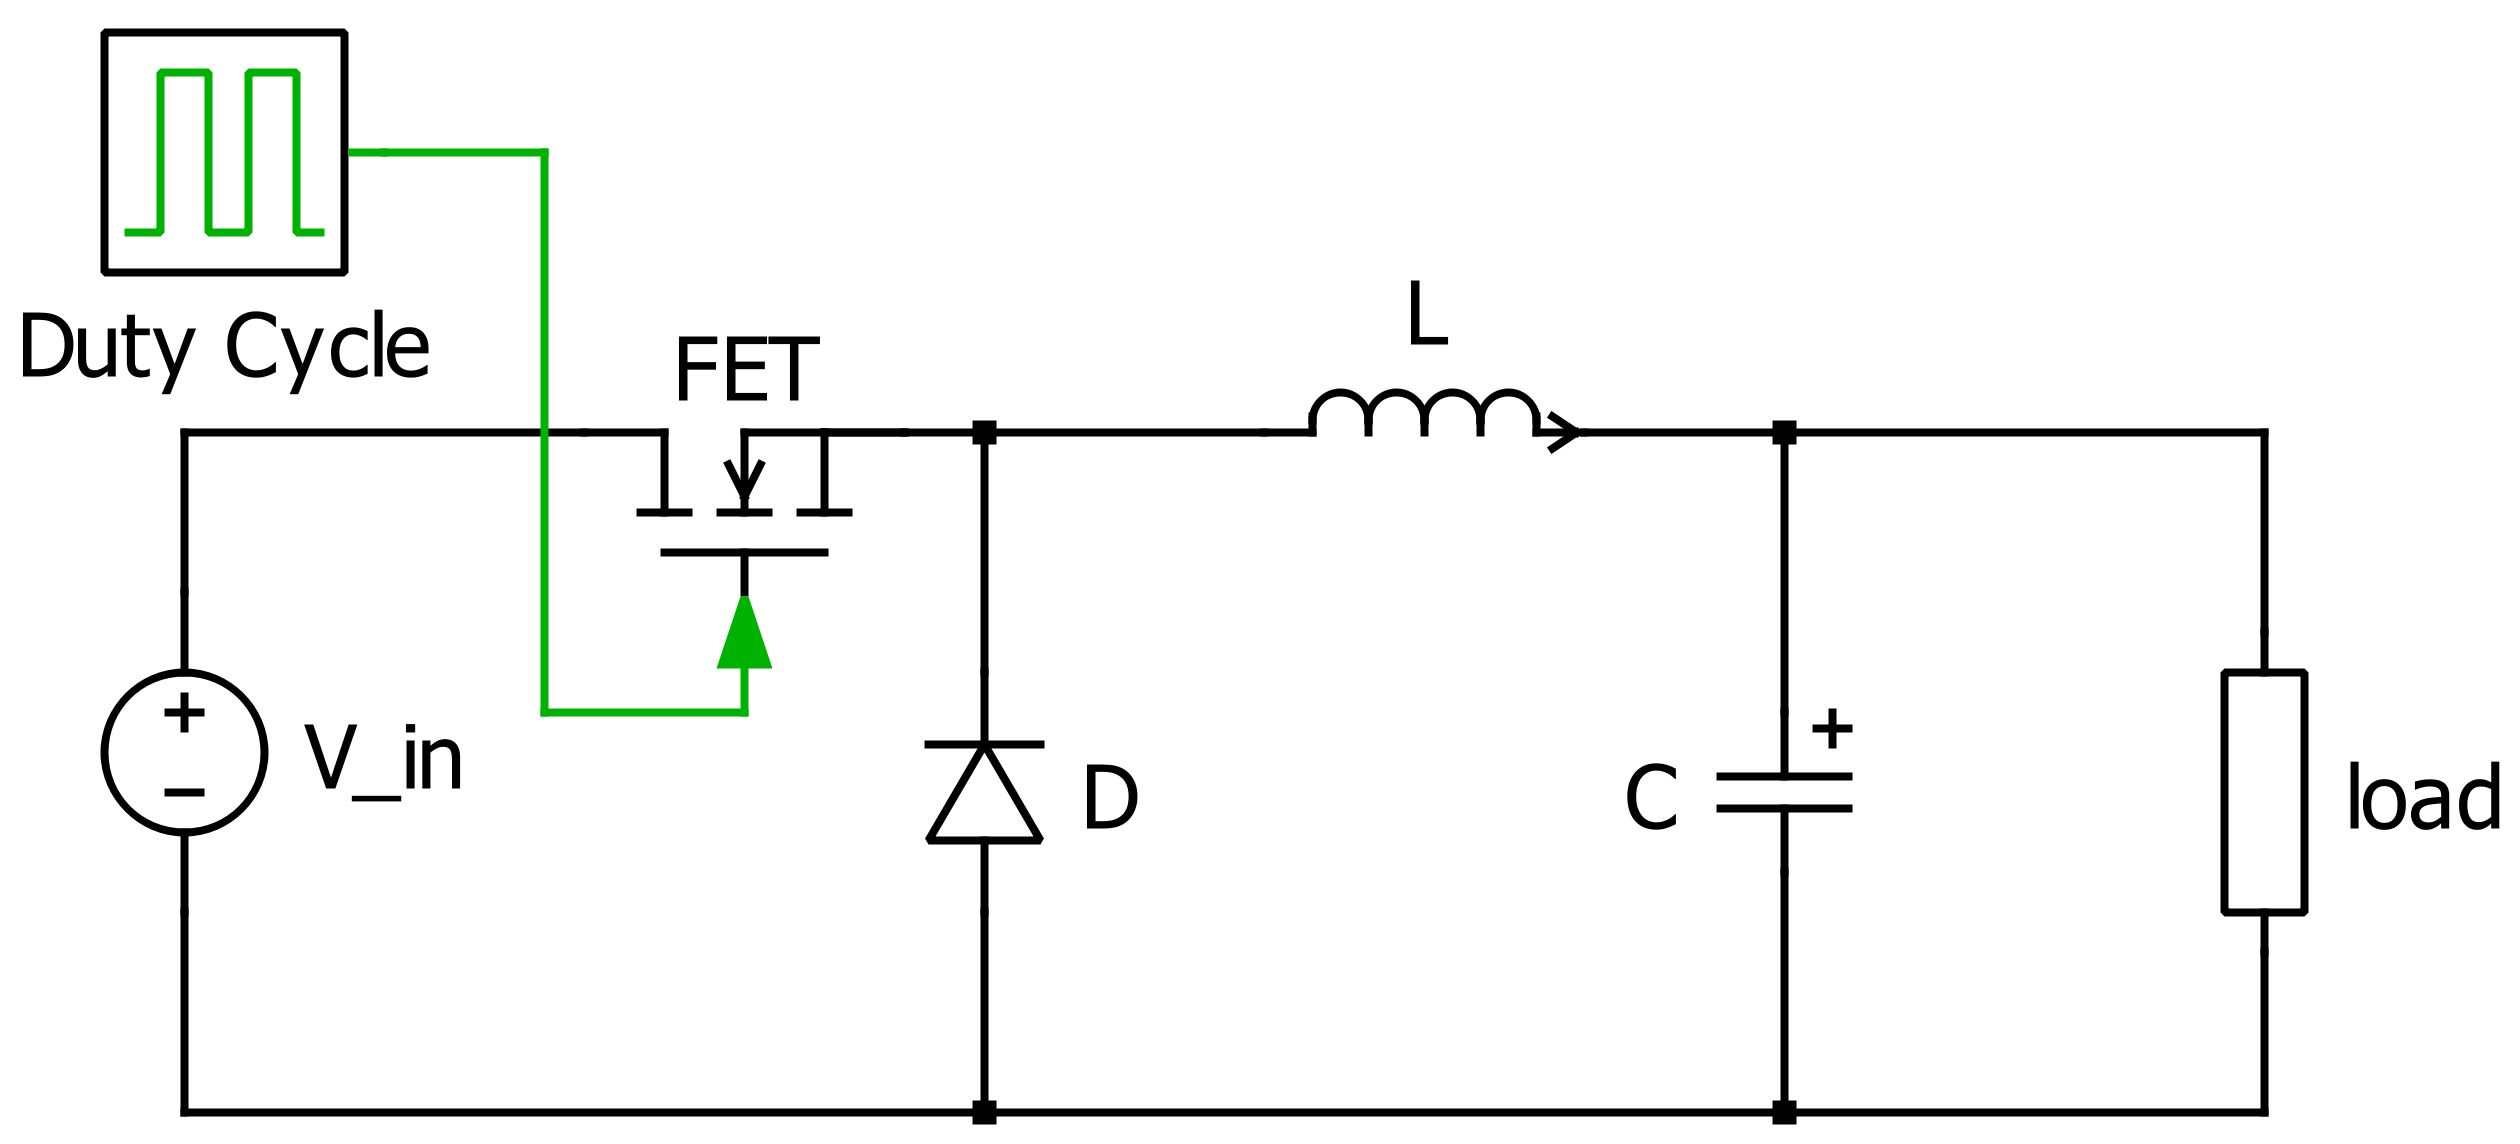
\includegraphics[width=0.7\textwidth]{../Pictures/Buck-converter}
		\caption{Buck-converter.}
		\label{Buck-converter}
	\end{center}	
\end{figure}

A buck-converter performs in two operating states. 
During the first state, the MOSFET is conducting and the diode is working as an open-circuit, the voltage drop  then is divided between the inductor and load. Since the voltage is split, the voltage drop on the load is lower than the one of the input source. In addition, both the capacitor and the inductor are being charged. In the second state, the MOSFET is switched off and the current flows through the diode. During this state, the inductor works as a current source and the capacitor stabilizes the voltage \cite{schematicbuckandboost}.

The main advantage for using the buck converter is that the structure is very simple and only one controlled  switch is needed. Also, the component count and thus cost of components is low. Furthermore, the buck converter can reach efficiencies up to 99\% \cite{Efficiencybuck}. 

However, this topology is not very versatile since it does not allow the increase of output voltage with respect to the input. Another drawback is the lack of galvanic isolation between the input and the output \cite{advantagebuck}.
%%http://www.completepowerelectronics.com/buck-converter-tutorial-topology-working-advantages-applications/

\section{Boost converter\label{Boost-C}}

A boost converter is another type of DC-DC converter, it is similar to the buck but instead of lowering the output voltage, it produces a higher electrical potential at the output with respect to that at the input.

The circuit consists of two switches (a transistor and a diode), an inductor, a capacitor, a load and a DC-source for the input voltage. Figure \ref{Boost-converter} shows an equivalent circuit diagram with the aforementioned components. %%\cite{Reddy2011}

\begin{figure}[htbp]
	\begin{center}
		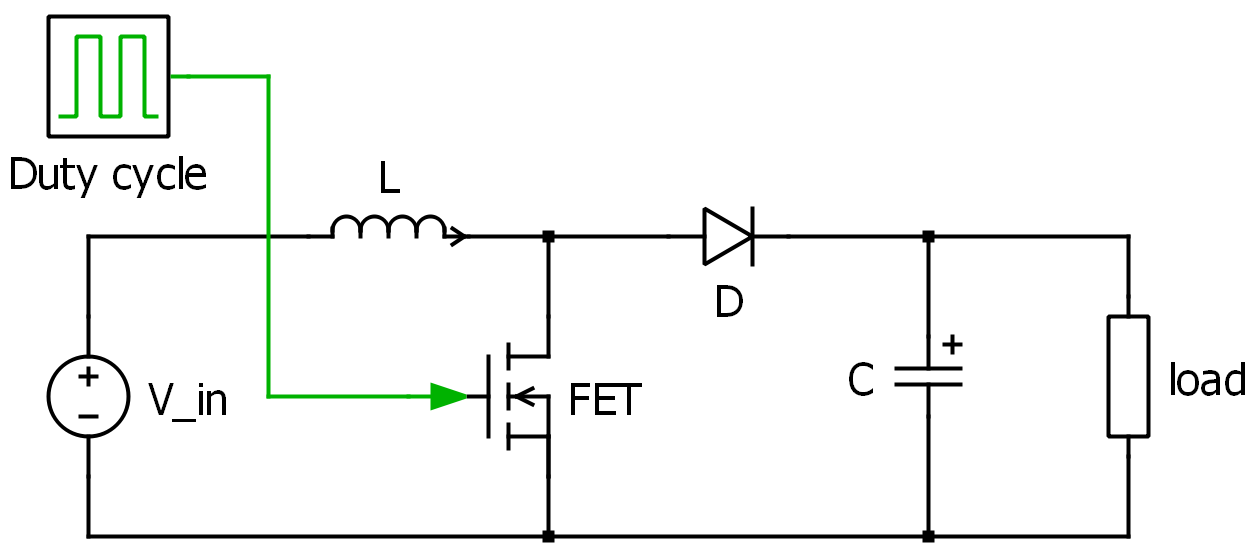
\includegraphics[width=0.7\textwidth]{../Pictures/Boost-converter}
		\caption{Boost-converter.}
		\label{Boost-converter}
	\end{center}	
\end{figure}

Similarly to the buck converter, this topology has two states, when the MOSFET is on, the current flows only trough the inductor because the diode  is working as an open-circuit. Energy is then stored in the inductor, which voltage is equal to the input voltage, and current increases. Meanwhile, the capacitor releases the previously stored energy to the load.
During the second state, the MOSFET is turned off, the current then loops trough the inductor, diode, capacitor and the load. Since the inductor had been previously charged, it now works as a current source in series with the voltage source of the circuit. The voltage across the load is then risen with respect to that at the input. Furthermore, the capacitor is charging \cite{schematicbuckandboost}.

An advantage for a boost converter is that it can raise the output voltage without using a transformer. It is also a cheap converter easy to control \cite{advantageboost}. 

However, as it happened with the buck, the boost converter is also limited to rising the voltage and lowering it cannot be achieved. Also, if an error happens in the control of the MOSFET and it is left in ON-mode for a long time, a short-circuit is created and the current will increase until a component fails. Finally, this converter does not have galvanic isolation either. 
 
